\documentclass[a4paper,11pt]{report}
\usepackage[a4paper]{geometry}
\usepackage[english]{babel}
\usepackage{graphicx,subfigure}


\author{Cedric~Cuypers, Kenzo~Tomita, Guy~Van~den~broeck} 
% define title
\title{Ontwerp en Analyse van Software Systemen II: a~poker~application} 
\begin{document} 
% generates the title 
\maketitle 
% insert the table of contents 
\tableofcontents 
\chapter{Introduction}
\chapter{Business goals}

\section{Business environment}
\subsection{History}
The game of poker dates back to as early as 1890. It became popular as a casino game around 1970. In 1987, community card poker games were introduced. These games proved far more exciting than the draw poker variants that were played up until that time. The game got more complex and required more skilful players. Poker became part of popular culture with the advent of movies and television programs about casino poker.

Recently, online poker has been partly responsible for a dramatic increase in the number of poker players worldwide. Hole-card cameras at big tournaments turned poker in to a spectator sport.

\subsection{Online poker}
Poker is very suitable for online play as casinos are intimidating for novice players and due to legal restictions only present in certain areas. Traditional casinos make money by asking a time fee or a rake (a percentage of the money won), but have high costs for setting up a table. Online poker rooms don't have that cost and can offer a large amount of tables with low rakes. They also offer tables with low stakes, where less wealthy or novice players can play or free tournaments where they can introduce people to the game.
Profit in online poker is made through a rake (as in real casinos), through an entry fee, through low interest rates on money deposited with the poker company or simply through advertisement. In the latter case, it is possible to only allow games for imaginary money or other virtual credits. 

The very small profit margin in real casino poker causes it to only be feasible for high stakes players. Online poker on a massive scale is the only profitable way to offer games for low stakes players.

There are a number of differences between online and offline play with respect to the game itself.
\begin{itemize}
 \item Online games are faster paced. Brick and mortar casinos average 30 hands per hour. Online casinos can average 90 or 100.
 \item Offline games allow you to observe your opponent's behaviour in more detail (such as body language).
 \item Online games are more mathematical.
 \item Advanced players often play multiple online games simultaneously to increase their profit.
\end{itemize}

\subsection{Stakeholders}
The following main stakeholders are identified in online poker:
\begin{description}
 \item[Online Casino] This is the company offering the possibility for people to play poker on their infrastructure. They are trusted by the players to keep certain aspects of the game secret and to handle the money in circulation safely.
 \item[Advertisers] This is the organization to which exposure is sold. They are a source of revenue for the Online Casino. Typically they can be unaware of the poker context in which their advertisements are shown or they can mine the data provided by the Online Casino to specifically target certain people and situations. More often than not they don't deal with the Online Casino directly but operate through a third party.
 \item[Players] These are the people playing poker.
 \end{description}

\section{Legal constraints}
Event though poker is not a game of pure chance and skilful players are easy to distinguish from bad players, gambling laws do apply to poker in most countries. Online poker is legal in some countries but strongly regulated. Many banks are not allowed to transfer money to online poker sites. The legality of playing on a foreign poker site is unclear in most jurisdictions that don't allow gambling.

All these rules obviously don't apply to online poker games that use virtual money and get their revenue from advertisement.

\section{Business and technical constraints}

\subsection{Business goals}
Based on the previous discussion, we can now easily enumerate the primary business goals for the Online Casino.
 Primary business goals:
\begin{itemize}
\item Being attractive to paying advertisers
\item Being attractive to paying players or players that are interesting for the advertiser
\end{itemize}

Aside from the primary goals, secondary goals exist. Each of these goals can directly be traced back to 
the primary goals.

Secondary business goals:
\begin{itemize}
\item Ease of management: By automating internal management processes (customer management, accounting), internal efficiency can be optimized, and operational costs can be minimized. 
\item Ease  of  advertisement:  Ideally the software helps the advertiser to optimize its advertisements (e.g. by helping adding relevant meta�data).
\item Advertisement   feedback:   It   is   very   interesting   for   advertisers   to   consult   advertisement statistics, as these provide them a measure for the success of their advertisement campaign. These statistics could include: the percentage of all players that have seen the advertisement, the 
  profile of an average player that had interest in the advertisement, etc. 
\item User experience: Ensuring that the user experience is state�of�the�art. This includes a graphically appealing interface for the player, fast response times and good availability. Alternative online casinos are only a click away when the user is upset.
\item Assurance   of   customer   data   confidentiality:   Due   to   legislative   privacy   regulations,   the confidentiality of both types of customers data (players and advertisers) needs to be assured at all times. It must for example not be possible for advertisers to derive which exact players have seen their advertisements. Gambling isn't legally or socially accepted everywhere, so it is best kept private.
\item Assurance that the game is fair, that no parties have inside information or that cheating is happening in any form.
\end{itemize}

\chapter{Analysis}
\section{Domain Model}
See Figure \ref{fig:domain}.
\begin{figure}
  \begin{center}
    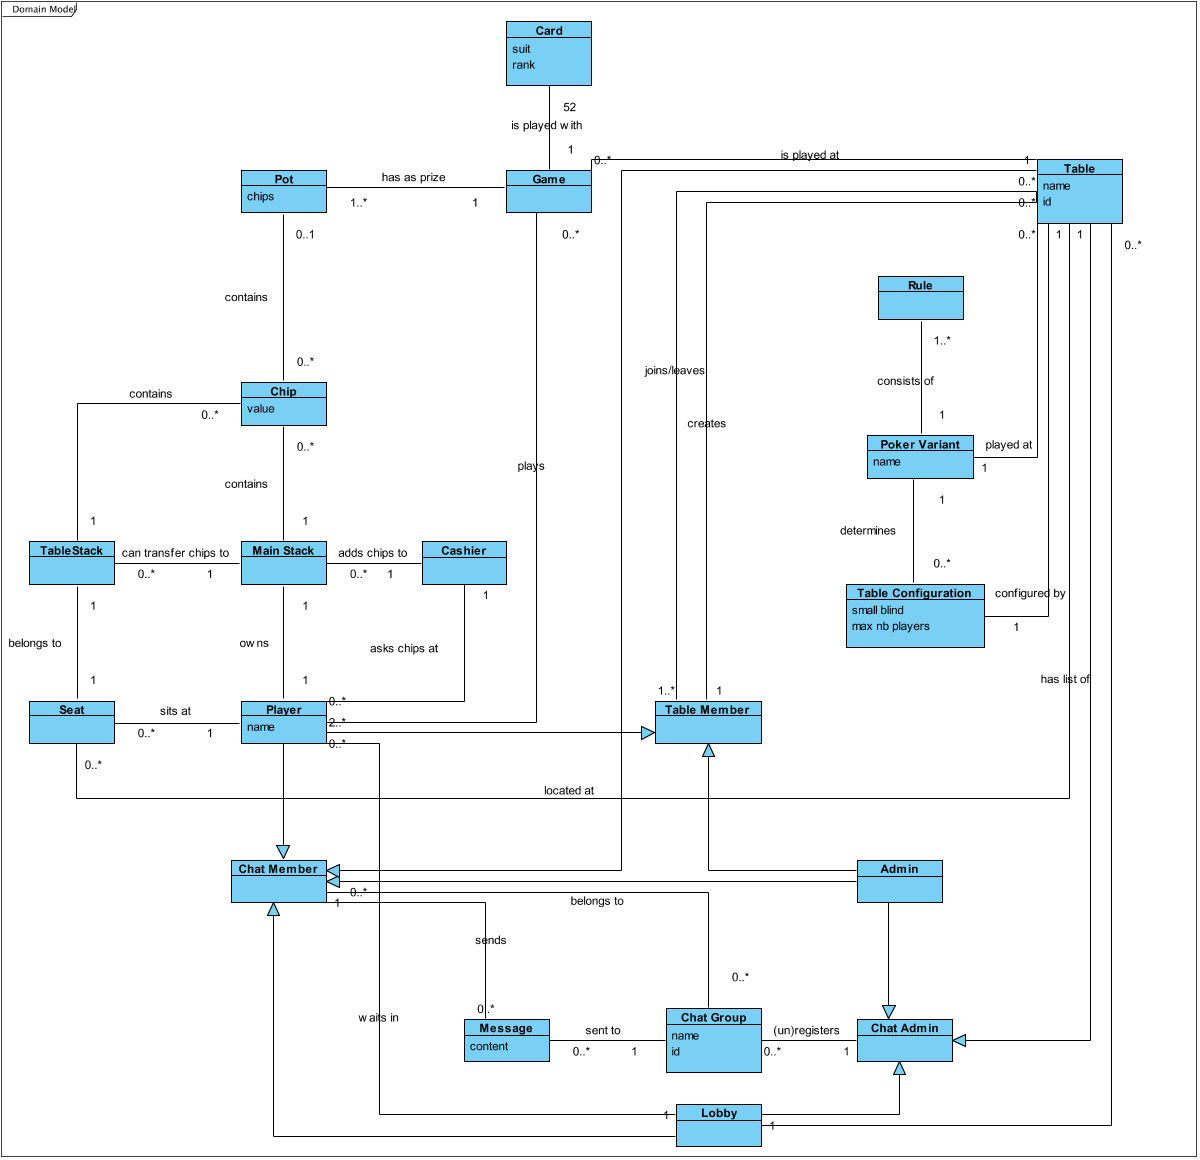
\includegraphics[scale=0.5]{img_domain_model.png}
  \end{center}
  \caption{Domain Model}\label{fig:domain}
\end{figure}
\section{Stakeholders and Actors}
TODO Guy
\section{Informal set of requirements}
\section{Available Use Cases}
\subsection{Create table}
\textbf{Level:} user goal \\
\textbf{Primary Actors:} Player, Admin \\
\textbf{Stakeholders:} This player and other players.\\
\textbf{Preconditions:} The player is logged-in.\\
\textbf{Success Guarantee:} A new table with given configuration is created. \\
\textbf{Main success scenario:} 
\begin{enumerate}
\item The actor selects to create a new table.
\item The system asks for a name for the table.
\item The actor enters a name for the table.
\item The system proposes a number of available poker variants (e.g. Texas hold'em, Omaha hold'em, ...)
\item The actor selects a poker variant. 
\item The system asks for a table configuration for the chosen poker variant.
\item The actor provides the system with a table configuration\footnote{A table configuration depends on the poker variant chosen. This could include the value of the blinds, bets, maximum number of players, auto-deal, minimal delay between 2 deals, ...}.
\item The system creates a new table. 
\item The system registers a new chat group for this table: \emph{\underline{Register chat group}}
\item The system informs the actor the table is created.
\item The system joins the actor to the table:  \emph{\underline{Join table}}
\end{enumerate}
\textbf{Extensions:}
\begin{itemize}
\item[3a.] The given name is not valid.
\begin{enumerate}
\item The actor can choose to retry (go to step 2) or to end the use case. 
\end{enumerate}
\item[7a.] The given table configuration is not valid. 
\begin{enumerate}
\item The actor can choose to retry (go to step 6) or to end the use case. 
\end{enumerate}
\end{itemize}
\subsection{Show table list}
\textbf{Level:} user goal \\
\textbf{Primary Actors:} Player, Admin \\
\textbf{Stakeholders:} \\
\textbf{Preconditions:} The player is logged-in.\\
\textbf{Success Guarantee:} A detailed list with the existing tables is shown.\\
\textbf{Main success scenario:} 
\begin{enumerate}
\item The actor selects to show the table list.
\item The system shows a detailed table list.
\end{enumerate}

\subsection{Join table}
\textbf{Level:} user goal \\
\textbf{Primary Actors:} Player, Admin \\
\textbf{Stakeholders:} \\
\textbf{Preconditions:} The player is logged-in.\\
\textbf{Success Guarantee:} The joined player receives the table events. \\
\textbf{Main success scenario:} 
\begin{enumerate}
\item The actor selects a table to join. 
\item The system registers the actor at the table. 
\item The system informs other joined users a new actor has joined the table.
\item The system informs the actor he is joined at the table.
\item The system informs the actor of new table events.
\end{enumerate}
\textbf{Extensions:}
\begin{itemize}
\item[1a.] The player is already joined at this table.
\begin{enumerate}
\item The system informs the actor he is already joined at this table.
\item The actor can try this step with an other table, or end the use case.
\end{enumerate}
\end{itemize}

\subsection{Leave table}
\textbf{Level:} user goal \\
\textbf{Primary Actors:} Player, Admin \\
\textbf{Stakeholders:} \\
\textbf{Preconditions:}
\begin{itemize}
\item The actor is logged-in.
\item The actor is joined at the table.
\end{itemize}
\textbf{Success Guarantee:} The actor is no longer joined at the table. \\
\textbf{Main success scenario:} 
\begin{enumerate}
\item The actor selects the option to leave the table.
\item The system unregisters the actor from the table.
\item The system informs the actor he has left the table. 
\item The system informs all other joined players the actor has left. 
\item The system does no longer inform the actor in case of table events.
\end{enumerate}
\textbf{Extensions:}
\begin{itemize}
\item[1a.] The selected person is sit-in at the table. 
\begin{enumerate}
\item The system performs a sit-out for the player: \emph{\underline{Sit-out}}
\item The actor can try this step with an other seat, or end the use case.
\end{enumerate}
\end{itemize}

\subsection{Sit-in}
\textbf{Level:} user goal \\
\textbf{Primary Actor:} Player \\
\textbf{Stakeholders:} \\
\textbf{Preconditions:}
\begin{itemize}
\item The player is logged-in.
\item The player is joined at the table.
\end{itemize}
\textbf{Success Guarantee:} The player can act in the game.\\
\textbf{Main success scenario:} 
\begin{enumerate}
\item The actor selects a seat to sit in. 
\item The system asks for the buy-in amount for this table. 
\item The actor enters the buy-in amount. 
\item The system transfers the buy-in amount from the actors main stack to his table stack.
\item The system registers the actor as a player at this table. 
\item The system informs the actor he is sit-in at the table.
\end{enumerate}
\textbf{Extensions:}
\begin{itemize}
\item[1a.] The selected seat does not exist or is already taken.
\begin{enumerate}
\item The system informs the actor the seat does not exist or is already taken.
\item The actor can try this step with an other seat, or end the use case.
\end{enumerate}
\item[1b.] The player is already sit-in at this table.
\begin{enumerate}
\item The system informs the actor he is already sit-in at this table.
\item The use case ends.
\end{enumerate}
\item[3a.] The entered amount is not valid. 
\begin{enumerate}
\item The system informs the actor the entered amount is not valid.
\item The actor can try this step with an other amount, or end the use case.
\end{enumerate}
\end{itemize}

\subsection{Sit-out}
\textbf{Level:} user goal \\
\textbf{Primary Actor:} Player \\
\textbf{Stakeholders:} \\
\textbf{Preconditions:}
\begin{itemize}
\item The player is logged-in.
\item The player is sit-in at the table.
\end{itemize}
\textbf{Success Guarantee:} The player can no longer act in the game.\\
\textbf{Main success scenario:} 
\begin{enumerate}
\item The actor selects the option to sit-out the table.
\item The system unregisters the actor as a player at this table. 
\item The system transfers the table stack back to his main stack. 
\item The system informs the actor he is no longer sit-in at the table. 
\item The system informs all other joined users the actor is no longer sit-in at the table.
\end{enumerate}
\textbf{Extensions:}
\begin{itemize}
\item[2a.] The player is active in the current deal.
\begin{enumerate}
\item The system folds for the player: \emph{\underline{Fold action}}
\end{enumerate}
\end{itemize}

\subsection{Table action (bet, raise, call or check)}
\textbf{Level:} user goal \\
\textbf{Primary Actor:} Player \\
\textbf{Stakeholders:} \\
\textbf{Preconditions:}
\begin{itemize}
\item The player is logged in.
\item The player is sit-in at the table.
\end{itemize}
\textbf{Success Guarantee:} The selected action is performed. \\
\textbf{Main success scenario:} 
\begin{enumerate}
\item The actor selects to bet, raise, call or check. 
\item The system performs the selected action. 
\item The system informs all other joined users the actor has performed an action at the table.
\end{enumerate}
\textbf{Extensions:}
\begin{itemize}
\item[1a.] The player chooses to bet or raise. 
\begin{enumerate}
\item The system aks for an amount.
\item The actor enters the amount. 
\item The system registers the action with the given amount.
\end{enumerate}
\item[1b.] It's not the turn of the player. 
\begin{enumerate}
\item The system informs the player it's not yet his turn. 
\item The use case ends.
\end{enumerate}
\item[1c.] The action the player tries to perform is not valid. 
\item[1d.] The player does not choose an action quick enough and a time-out occurs.
\begin{enumerate}
\item The system folds for the player: \emph{\underline{Fold action}}
\item The use case ends.
\end{enumerate}
\end{itemize}

\subsection{Fold action}
\textbf{Level:} user goal \\
\textbf{Primary Actor:} Player \\
\textbf{Stakeholders:} \\
\textbf{Preconditions:}
\begin{itemize}
\item The player is logged in.
\item The player is sit-in at the table.
\end{itemize}
\textbf{Success Guarantee:} The player folds. \\
\textbf{Main success scenario:} 
\begin{enumerate}
\item The actor selects fold.
\item The system performs the fold action. 
\item The system informs all other joined users the actor has folded at the table.
\end{enumerate}

\subsection{Show table information}
\textbf{Level:} user goal \\
\textbf{Primary Actor:} User \\
\textbf{Stakeholders:} \\
\textbf{Preconditions:}
\begin{itemize}
\item The user is logged in.
\end{itemize}
\textbf{Success Guarantee:} The table information is shown to the actor. \\
\textbf{Main success scenario:} 
\begin{enumerate}
\item The actor selects the option to show table information. 
\item The system asks to choose the table. 
\item The actor chooses the table to show the information from.
\item The system shows the table information\footnote{The table information consists of table id, name, a list of sit-in players, playing status and the table configuration.}. 
\end{enumerate}

\subsection{Register chat group}
\textbf{Level:} subfunction \\
\textbf{Primary Actor:} Other subsystem, Admin \\
\textbf{Stakeholders:} The players who want to use the chat service to chat. \\
\textbf{Preconditions:} none \\
\textbf{Success Guarantee:} A new chat group is registered. \\
\textbf{Main success scenario:} 
\begin{enumerate}
\item The actor chooses the option to register a new chat group. 
\item The chat system asks for a name for the chat group. 
\item The actor gives a name to the chat group. 
\item The chat system returns a handler to send/receive messages from the newly created chat group. 
\end{enumerate}
\textbf{Extensions:}
\begin{itemize}
\item[3a.] The given name is invalid.
\begin{enumerate}
\item Actor can choose to retry (go to step 2) or to end the use case. 
\end{enumerate}
\end{itemize}

\subsection{Unregister chat group}
\textbf{Level:} subfunction \\
\textbf{Primary Actor:} Other subsystem, Admin \\
\textbf{Stakeholders:}  \\
\textbf{Preconditions:} none \\
\textbf{Success Guarantee:} A new chat group is registered. \\
\textbf{Main success scenario:} 
\begin{enumerate}
\item The actor chooses the option to unregister a chat group. 
\item The chat system asks for an id of the chat group to unregister.
\item The actor provides an id to the chat system. 
\item The chat system unregisters the relevant chat group. 
\end{enumerate}
\textbf{Extensions:}
\begin{itemize}
\item[3a.] The given id is invalid.
\begin{enumerate}
\item Actor can choose to retry (go to step 2) or to end the use case. 
\end{enumerate}
\end{itemize}

\subsection{Send a message to a chat group}
\textbf{Level:} subfunction \\
\textbf{Primary Actors:} Table subsystem, Lobby subsystem, Player, Admin \\
\textbf{Stakeholders:}  \\
\textbf{Preconditions:} none \\
\textbf{Success Guarantee:} The message is sent to the chat group.  \\
\textbf{Main success scenario:} 
\begin{enumerate}
\item The actor chooses the option to send a message to a chat group. 
\item The chat system asks for an id of the chat group. 
\item The actor provides an id to the chat system.
\item The chat system asks to enter a message. 
\item The actor enters the message.
\item The chat system sends the message to all the players subscribed to the chat group.
\end{enumerate}
\textbf{Extensions:}
\begin{itemize}
\item[3a.] The given id is invalid.
\begin{enumerate}
\item Actor can choose to retry (go to step 2) or to end the use case. 
\end{enumerate}
\item[5a.] The entered message is not valid. 
\begin{enumerate}
\item Actor can choose to retry (go to step 4) or to end the use case. 
\end{enumerate}
\end{itemize}

\subsection{Login}
\textbf{Level:} user goal \\
\textbf{Primary Actor:} User \\
\textbf{Stakeholders:} \\
\textbf{Preconditions:} none \\
\textbf{Success Guarantee:} The player is logged in.\\
\textbf{Main success scenario:} 
\begin{enumerate}
\item The actor selects to login. 
\item The system asks for a user name and password. 
\item The actor enters his user name and password.
\item The system authenticates the actor. 
\item The system puts the actor in the lobby. 
\item The system informs the actor he is logged in. 
\end{enumerate}
\textbf{Extensions:}
\begin{itemize}
\item[4a.] The system fails to authenticate the actor (user name - password combination is incorrect, user blocked, ...). 
\begin{enumerate}
\item Actor can choose to retry (go to step 2) or to end the use case. 
\begin{enumerate}
\item[1a.] The actor has tried to authenticate himself more often than a predefined threshold.
\begin{enumerate}
\item[1.] The system denies the actor to proceed the use case for a period of time.
\end{enumerate}
\end{enumerate}
\end{enumerate}
\end{itemize}

\subsection{Logout}
\textbf{Level:} user goal \\
\textbf{Primary Actor:} User \\
\textbf{Stakeholders:} \\
\textbf{Preconditions:} The player is logged in. \\
\textbf{Success Guarantee:} The player is logged out.\\
\textbf{Main success scenario:} 
\begin{enumerate}
\item The actor selects to logout. 
\item The system removes the actor from all the tables he is joined to: \emph{\underline{Leave table}}
\item The system stores the state of the player.
\item The system clears all actor related data. 
\item The system informs the actor he is logged out. 
\end{enumerate}

\subsection{Create account}
\textbf{Level:} user goal \\
\textbf{Primary Actor:} User \\
\textbf{Stakeholders:} \\
\textbf{Preconditions:} \\
\textbf{Success Guarantee:} A new account is created. \\
\textbf{Main success scenario:} 
\begin{enumerate}
\item The actor selects to create a new account. 
\item The system asks for a user name and password.
\item The actor enters the user name and password (twice to exclude typos).
\item The system creates a new account with given credentials. 
\item The system informs the actor the account is created.
\end{enumerate}
\textbf{Miscellaneous:} user information could also mean an emailadres for confirmation or a captcha.

\subsection{Request chips}
\textbf{Level:} user goal \\
\textbf{Primary Actor:} Player \\
\textbf{Stakeholders:} \\
\textbf{Preconditions:} The player is logged in. \\
\textbf{Success Guarantee:} The player receives a number of chips to its main stack. \\
\textbf{Main success scenario:} 
\begin{enumerate}
\item The actor selects to request a number of chips. 
\item The system asks for the number of chips. 
\item The actor enters an amount. 
\item The system asks for a payment method. 
\item The actor chooses the payment method. 
\item The system redirects to a 3rd party component to perform the payment.
\item The actor enters all necessary information asked by the 3rd party component. 
\item The system performs the transaction. 
\item The system provides the player with the respective amount of chips. 
\end{enumerate}
\textbf{Extensions:}
\begin{itemize}
\item[*a.] At any time, player cancels the operation. 
\item[3a.] The amount is not valid. 
\begin{enumerate}
\item The system informs the actor the entered amount is invalid. 
\item The actor can choose to retry (go to step 2) or to end the use case. 
\end{enumerate}
\item[7a.] The transaction can not be performed because the entered information is invalid. 
\begin{enumerate}
\item The system informs the actor the transaction couldn't be performed. 
\item The actor can choose to retry (go to step 6), to choose another payment method (go to step 4) or to end operation. 
\end{enumerate}
\end{itemize}

\chapter{Architecture: Functional viewpoint}
The functional viewpoint presents the architectural elements needed to provide the core business of the poker application. This core business is translated into a core service, which is more specifically the service of providing poker tables. Additional issues needed to allow the poker company to perform its core business are also taken into account: account management, administration and cashier.

\section{Architecture Component Diagram}
This section identifies several main internal components. The component diagram (Figure~\ref{fig:component}) also identifies the main interfaces that can be used by the components to communicate with each other.

To give a better understanding of each of the internal components a brief overview of each component is provided with an explanation of their role and responsibilities within the architecture.

\begin{figure}
  \begin{center}
    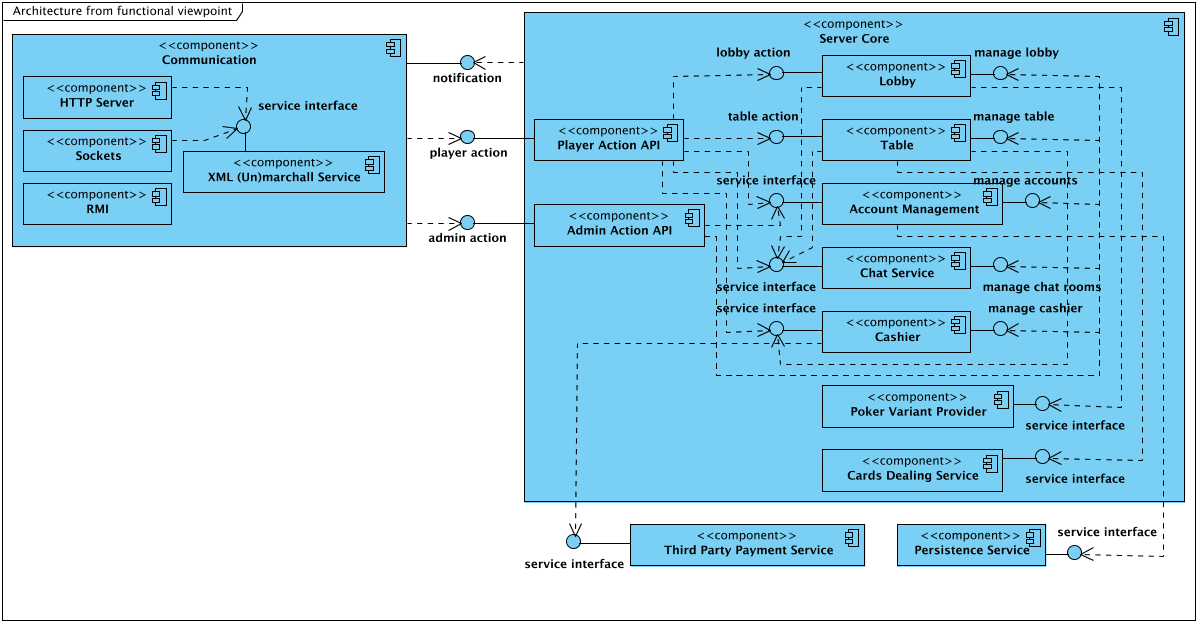
\includegraphics[angle=90, scale=0.6]{img_architecture_component_diagram.png}
  \end{center}
  \caption{Architecture from a functional viewpoint}\label{fig:component}
\end{figure}

\subsection{Lobby}
The lobby component is responsible for managing tables. It is a registry service for looking up existing tables. It is also the interface to create and register new tables. 
\subsubsection{Interfaces}
\begin{itemize}
\item \emph{lobby action}: This interface is used to handle lobby actions. This includes looking up tables, retrieving table information, creating tables, ...
\item \emph{manage lobby}: This interface provides an admin the possibility to perform lobby related management.
\end{itemize}

\subsection{Table}
The table component is responsible for handling player actions at a table. This component handles all the game play logic that is necessary to play a poker variant.
\subsubsection{Interfaces}
\begin{itemize}
\item \emph{table action}: This interface is used to handle table actions. This includes sit-in, sit-out, check,  call, bet, raise and fold.
\item \emph{manage table}: This interface provides an admin the possibility to perform table related management.
\end{itemize}

\subsection{Account Management}
The account management component is responsible for managing users. An account contains all user related data. It provides an interface to create, remove and block accounts. It also keeps track of the main stack each player has. This component interacts with the persistence component to store user data.
\subsubsection{Interfaces}
\begin{itemize}
\item \emph{manage my account}: This interface provides a user the possibility to modify his own account data such as name, password, avatar, ...
\item \emph{manage accounts}: This interface provides an admin the possibility to modify all account data. Additionally this interface is used to remove and block accounts. 
\item \emph{transfer chips}: This interface is used to transfer chips from and to the account of player.
\end{itemize}

\subsection{Cashier}
The cashier component is responsible for providing players with chips. If real money is involved, this component will interact with a third party payment component to exchange real money with chips. Otherwise any time-based function or admin functionality can provide players with chips through this component.
\subsubsection{Interfaces}
\begin{itemize}
\item \emph{service interface}: This interface is used to provide players with chips. 
\item \emph{manage cashier}: This interface is used by an admin to manage the functionality of the poker server.
\end{itemize}

\subsection{Chat Service}
The chat component is responsible for managing chat groups and delivering chat messages to other players. The chat component provides an interface to create and remove chat groups. The lobby and table components will use this functionality to provide chat services to the players in the respective components.
\subsubsection{Interfaces}
\begin{itemize}
\item \emph{service interface}: This interface is used to register a chat group and send messages to a chat group.
\item \emph{manage chat rooms}: This interface is used by an admin to manage the functionality of the poker server.
\end{itemize}

\subsection{Cards Dealing Service}
The cards dealing service component is responsible to provide securely shuffled cards to the table component.
\begin{itemize}
\item \emph{service interface}: This interface is used to retrieve and shuffle cards.
\end{itemize}

\subsection{Poker Variant Provider}
The poker variant provider component is responsible for managing and providing the available poker variants. A  poker table is always configured with a poker variant provided by this component.
\begin{itemize}
\item \emph{service interface}: This interface is used to look up a poker variant and retrieve the necessary configuration to play a chosen poker variant.
\end{itemize}

\subsection{Communication}
This component is responsible for the communication between client and server modules. It delegates API calls to the responsible component.
\begin{itemize}
\item \emph{notification}: This interface is used to send messages from the server core to the respective clients.
\end{itemize}

\subsection{Persistence Service}
This component is responsible for handling the persistence needs for all other components.
\begin{itemize}
\item \emph{notification}: This interface is used to store and retrieve data from the persistent storage.
\end{itemize}

\section{Use Cases applied on the component diagram}
\section{Deployment View}
The deployment view (Figure \ref{fig:deployment}) provides a mapping of the previously defined component instances onto the physical nodes in a computer network. 
\begin{figure}
  \begin{center}
    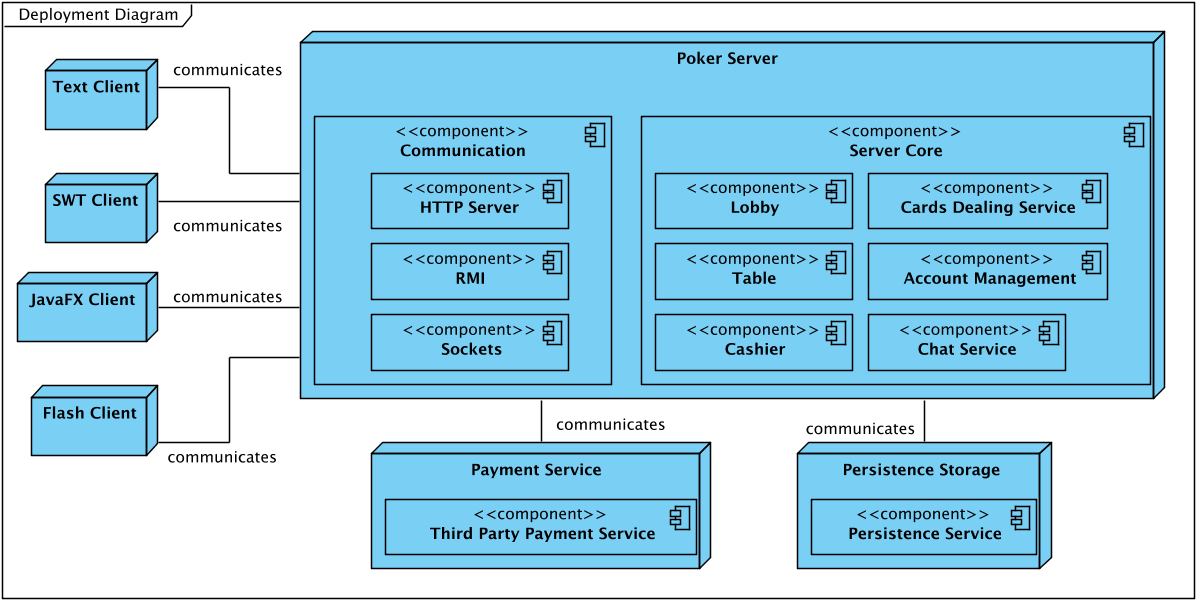
\includegraphics[angle=90, scale=0.6]{img_deployment_diagram.png}
  \end{center}
  \caption{Deployment Diagram}\label{fig:deployment}
\end{figure}

\end{document} 